\chapter{Case Study}


\section{Introduction}

\section{Problem formulation}
\begin{opt}
Consider the optimal placement problem of \(n\) mecanum robots moving on a plane, indexed by the set \(\mathcal{V} = \{1,\ldots,n\}\). Each robot has access to the Cartesian coordinates of a set of fixed anchor points, as well as information from its neighbors defined over an undirected communication graph \(\mathcal{G} \coloneqq (\mathcal{V}, \mathcal{E})\), where \(\mathcal{E}\subseteq \mathcal{V}\times\mathcal{V}\). An edge \((i,j)\in\mathcal{E}\) indicates that robots \(i\) and \(j\) can exchange information.

The objective is to design a \textbf{distributed control algorithm} that specifies the accelerations of the robots so that their positions converge to a configuration minimizing the cost function
\begin{equation}
\begin{split}
    f(\{p_x^i, p_y^i\}_{i\in\mathcal{V}}) 
    &= \frac{1}{2}\sum_{(i,j) \in \mathcal{E}} \Big((p_x^i - p_x^j)^2 + (p_y^i - p_y^j)^2\Big) \\
    &\quad + \frac{1}{2} \sum_{i\in\mathcal{V}} \sum_{(a_k,b_k)\in \mathcal{B}_i} \Big((p_x^i - a_k)^2 + (p_y^i - b_k)^2\Big),
\end{split}
\end{equation}
where \(\mathcal{B}_i\) denotes the set of anchor points available to robot \(i\).
\end{opt}


\begin{rem}
The problem admits a straightforward centralized solution by computing
\[
p^\star \coloneqq \arg \min f(p),
\]
and commanding all robots to move directly to their optimal positions. However, designing a distributed solution is nontrivial due to the following challenges:
\begin{itemize}
    \item The global cost function must be decomposed into local objectives that can be evaluated using only locally available information.
    \item Due to communication constraints and delays, each agent has access only to outdated or partial information about its neighbors, which introduces bias in the local evaluation of the cost.
    \item The robot dynamics impose physical constraints, preventing instantaneous velocity changes. Poorly designed control laws may therefore lead to oscillations, overshoot, or even instability.
    \item The aforementioned factors are intrinsically intertwined, making it difficult to establish a clear and well-defined separation among them.
\end{itemize}
\end{rem}

\begin{rem}
Mecanum robots are adopted in this simulation due to their ability to generate acceleration in arbitrary planar directions with minimal delay, which simplifies the dynamic modeling. The dynamical model of each robots is:
\begin{equation}
\begin{bmatrix}
    \dot{p} \\ \dot{v} \\ \dot{a}
\end{bmatrix}
= 
\begin{bmatrix}
    \mathbf{0}_{2\times 2} & I_2 & \mathbf{0}_{2\times 2}   \\
    \mathbf{0}_{2\times 2} & \mathbf{0}_{2\times 2} & I_2 \\
    \mathbf{0}_{2\times 2} & \mathbf{0}_{2\times 2} & -\frac{1}{\tau}I_2
\end{bmatrix}
\begin{bmatrix}
    p \\ v \\ a
\end{bmatrix}
+ \begin{bmatrix}
    \mathbf{0}_{2\times 2} \\ \mathbf{0}_{2\times 2} \\ \frac{1}{\tau}I_2
\end{bmatrix} u.
\end{equation}
\(p\), \(v\) and \(a\) are vectors in \(\mathbb{R}^2\) corresponding to the position, velocity and acceleration.
\end{rem}

\section{Proposed solution}
\subsection{Cost decomposition}
Each agent is associated with a private optimization problem \(f_i\colon \mathbb{R}^d \mapsto \mathbb{R}\). In this paper, \(f_i\) usually takes a canonical quadratic form:
\[
f_i(x) \coloneqq x^\top H_i x^\top + b_i^\top x, H_i \succeq 0\in\mathbb{S}^{d\times d}.
\]
We seek to solve a convex optimization problem using a multi-agent network. In particular, these agents collaborate to find the optima of the following problem:
\begin{opt}\label{Prob::Cen}

\end{opt}

\subsection{Distributed consensus optimization}
It's well-known that Problem \ref{Prob::Cen} can be decomposed into \(n\) local optimization tasks, each one managed by one agent, accompanied with a consensus problem. Each agent maintains a local copy of the variable \(x\), denoted by \(x^i\), and updates it using the gradient of its private objective function \(f_i\). To ensure that all agents converge to a common optimizer of the global objective, agents exchange information with their neighbors over the communication network and iteratively adjust their local states toward consensus. Define the vertical concatenation of \(x^i\) as \(x_v =\ver[x^i] \in \mathbb{R}^{nd\times 1}\). Let \(f(x_v)\coloneqq \sum_{i = 1}^n f_i(x^i)\). The problem decomposition introduces a constraint \(x^1 = x^2 = \hdots = x^n\) enforced by \(\mathcal{L}_v x_v = \mathbf{0}\) and changes Problem \ref{Prob::Cen} into the following:
\begin{opt}\label{Prob::Dis}
\begin{equation}
    p_d^* \coloneqq \min \sum_{i = 1}^n f_i(x^i)
\end{equation}
subject to
\[
\mathcal{L}_v x_v = \mathbf{0}.
\]
\end{opt}
\(\mathcal{L}_v = \mathcal{L} \otimes I_d\), where \( \mathcal{L}\) is the in-degree Laplacian matrix of an arbitrary strongly connected graph. Here, we force \( \mathcal{L}\) to be the Laplacian of \(\mathcal{G}\). Given \(\mathcal{A} \coloneqq [a_{ij}]\), \(a_{ij} = 1\) if \((j,i) \in \mathcal{E}\) as the binary adjacency matrix of \(\mathcal{G}\), define the in-degree matrix \(\mathcal{D}_{in} = \diag[d_{ii}] = \diag[\sum_{j = 1}^n a_{ij}]\), then \(\mathcal{L} = \mathcal{D}_{in} - \mathcal{A}\).
It's well known that the rank of \(\mathcal{L}\) is always \(n - 1\).

By this configuration, let \(\mathcal{L}_{i,\colon} \) denote the i-th row of \(\mathcal{L}\). Then, \(\mathcal{L}_{i,\colon} x_v\) can be interpreted as the difference of \(x\) between agent \(i\) compared to its in-neighbors in \(\mathcal{G}\). Introduce the dual variable \(\eta\).
\begin{opt}\label{Prob::Primal}
\begin{equation}
    p_d^* \coloneqq \inf_{x_v} \sup_{\eta\in \mathbb{R}^{nd\times 1}} f(x_v) + \langle \eta, L x_v\rangle.
\end{equation}
\end{opt}
The Primal-Dual Gradient Descent method gives:
\begin{align}
x_v^ + &= x_v - \alpha (\nabla f(x_v) + L^\top \eta) \\
\eta^+ &= \eta + \beta L x_v
\end{align}

We identify this gradient descent paradigm as a dynamical system characterized by a state-space model. We stresses that the term
\begin{equation}
\begin{split}
x_v - \alpha \nabla f(x_v) & = \ver[x^i - \alpha \nabla f_i(x^i)] \\
& = (I_{nd} - \alpha \cdot \diag[H_i]) x_v - \alpha \ver[b_i] 
\end{split}
\end{equation}
is the consequence of gradient descent about every local cost. Denote \(H \coloneqq \diag[H_i]\).

\begin{rem}
The dynamical system reaches the equilibrium
\[
\begin{bmatrix}
\mathbf{1}_n \otimes p^* \\
\eta_{ss}
\end{bmatrix}
\]
asymptotically when the learning rate \(\alpha\) and \(\beta\) are chosen so that the matrix
\[
\begin{bmatrix}
    I_{nd} - \alpha H & -\alpha L^\top\\
    \beta L & I
\end{bmatrix}
\]
has spectrum in \((-1,1]\) and the algebraic multiplicity  of eigenvalue \(1\) is exactly \(d\). Inside, \(\eta_{ss}\) is a vector in the affine space of \(\{y\vert\mathcal{L}^\top y = - H (\mathbf{1}_n \otimes p^*) - \ver[b_i]\}\).
\end{rem}




To apply our knowledge in the domain of control theory to tackle those optimization problems, the first step is to formalize a reasonable optimal control problem. We start with the block diagram of the system.
\begin{figure}[hb]
    \centering
    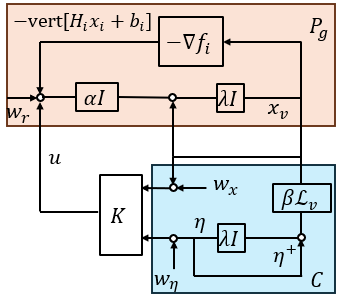
\includegraphics[width= 0.75\linewidth]{figures/CaseStudyFigs/DGDblkdiagram.png}
    \caption{}
\end{figure}


\(P_g\) is the block diagonal system that captures all the local gradient descent computations. \(C\) is a pre-processor that lets all agents gather information from in-neighbors and update \(\eta\). \(C\) is given by:
\[
C \coloneqq \begin{bmatrix}
    I \\
    \frac{1}{z - 1}\beta \mathcal{L}_v
\end{bmatrix}.
\]
Note that \(C\) has implicitly used the network for communication among agents.
\subsection{Generalized plant formulation}
We begin with the definition and explanation of selected input/output signals.

The measurement output \(y \coloneqq \ver[y_i]\). \(y_i\) at each agent consists of
\[
y_i = \begin{bmatrix}
    x_i \\
    \eta_i
\end{bmatrix}.
\]
The control input \(u \coloneqq \ver[u_i]\). \(u_i\) at each agent only serves to push \(x_i\) into consensus and doesn't engage into the acceleration of local gradient descent.
The exogenous disturbance output \(w\),
\[
w = \begin{bmatrix}
    w_r \\
    w_x \\
    w_\eta
\end{bmatrix}.
\]
\(w_r\) adds on the gradient vector, \(w_x\) that perturbs the states measurement, \(w_\eta\) that perturbs the \(\eta\) measurement. We can put appropriate weights on these noises to improve the performance of designed controller. The performance output \(z\) is given by
\[
z = \begin{bmatrix}
    \eta \\
    u \\
\end{bmatrix}.
\]
Some weights can be assigned to balance emphasis between \(u\) and \(\eta\). Especially, forcing \(T_{w_r \eta}\) as a bounded operator enables the controller to drive the term \(\mathcal{L}_v x_v\) asymptotically converges to \(\mathbf{0}\) and thus lets all agents reach consensus.
The state-space representation is given by:
\begin{equation}
\begin{split}\label{eqn::ss_sys}
\begin{bmatrix}
    x_v^ + \\
    \eta^+ 
\end{bmatrix}
& = \begin{bmatrix}
    I_{nd} - \alpha H & \mathbf{0}\\
    \beta \mathcal{L}_v & I
\end{bmatrix} 
\begin{bmatrix}
    x_v \\
    \eta 
\end{bmatrix} + \begin{bmatrix}
    \alpha I\\
    \mathbf{0}
\end{bmatrix} w_r +  \begin{bmatrix}
    \alpha I\\
    \mathbf{0}
\end{bmatrix} u \\
z & = \begin{bmatrix}
    \mathbf{0} & I\\
    \mathbf{0} & \mathbf{0} 
\end{bmatrix} \begin{bmatrix}
    x_v \\
    \eta 
\end{bmatrix} 
+ 
\begin{bmatrix}
    \mathbf{0}\\
    \gamma_1 I
\end{bmatrix} u \\
y & = 
\begin{bmatrix}
    I & \mathbf{0}\\
    \mathbf{0} & I
\end{bmatrix} \begin{bmatrix}
    x_v \\
    \eta 
\end{bmatrix}
+ \begin{bmatrix}
    \gamma_2 I & \mathbf{0}\\
    \mathbf{0} & \gamma_3 I
\end{bmatrix}
\begin{bmatrix}
    w_x \\
    w_\eta 
\end{bmatrix}
\end{split}   
\end{equation}
In the Primal-dual Gradient Descent, the control input \(u = - \mathcal{L}_v^\top \eta\) contributes to push \(x_v\) into consensus. In particular, the \(L^\top = L_0^\top \otimes I_d\) enforces that \((\mathbf{1}^\top \otimes I_d) u =\mathbf{0}\). Our goal is to redesign a control policy \(K\colon [x_v^\top,\eta^\top]^\top \mapsto u\) such that \((\mathbf{1}^\top \otimes I_d) u[t]\) is satisfied at any time. Toward this end, we require that \(K\in \mathcal{S}_c\), \(\mathcal{S}_c \coloneqq \{K\vert(\mathbf{1}^\top \otimes I_d)^\top K = \mathbf{0}\}\). 

We define the structured set as
\[
\mathcal{S}_\mathcal{G}\coloneqq \{K\vert KC \in \mathfrak{T}(\mathcal{G},\mathcal{P}_u,\mathcal{P}_{x_v})\},
\]
where \(\mathcal{P}_u = \mathcal{P}_{x_v} = d\mathbf{1}_n\). \(\mathcal{S}_\mathcal{G}\) captures that \(KC\) is a network distributed controller subject to the communication constraints introduced by the graph. 


\subsection{Model Reduction}
This state-space presented in (\ref{eqn::ss_sys}) is observable but always not fully controllable. The uncontrollable eigenvalue is \(\lambda = 1\) and the uncontrollable subspace is:
\[
\left\{
\begin{bmatrix}
    \mathbf{0}\\ v
\end{bmatrix}\vert 
v \in \ker(\mathcal{L}_v) = \mathbf{1}\otimes \mathbb{R}^d\right\} .
\]
\begin{rem}
The uncontrollable subspace fundamentally means the consensus control input can't shift all \(\eta_i\)s in one direction.    
\end{rem}
We find \(U\) to be the basis of the vector space \(\mathbb{R}^{nd} \times \im(\mathcal{L}_v)\). And let:
\begin{equation*}\small
\begin{split}
& P = \left[ \begin{array}{c:c}
    P_{11} & P_{12}\\
    \hdashline
    P_{21} & P_{22}
    \end{array}\right] \coloneqq \left[
\begin{array}{c|cc}
    A & B_w & B_u \\
    \hline
    C_z & D_{zw} & D_{zu} \\
    C_y & D_{yw} & D_{yu}
\end{array}\right] \\ 
& =
\left[
\begin{array}{c|cc}
    U^\top \begin{bmatrix}
    I_{nd} - \alpha H & \mathbf{0}\\
    \beta \mathcal{L}_v & I
    \end{bmatrix} U
    & U^\top \begin{bmatrix}
    \alpha I & \mathbf{0} & \mathbf{0}\\
    \mathbf{0} & \mathbf{0} & \mathbf{0}
    \end{bmatrix} & U^\top  \begin{bmatrix}
    \alpha I\\
    \mathbf{0}
    \end{bmatrix} \\
    \hline
    \begin{bmatrix}
    \mathbf{0} & I\\
    \mathbf{0} & \mathbf{0} 
    \end{bmatrix} U & \mathbf{0} & \begin{bmatrix}
    \mathbf{0}\\
    \gamma_1 I
    \end{bmatrix} \\
    \begin{bmatrix}
    I & \mathbf{0}\\
    \mathbf{0} & I
    \end{bmatrix} U & \begin{bmatrix}
    \mathbf{0} & \gamma_2 I & \mathbf{0}\\
    \mathbf{0} & \mathbf{0} & \gamma_3 I
\end{bmatrix} & \mathbf{0}
\end{array}\right]. 
\end{split}
\end{equation*}
This reduced state-space is controllable and observable. We design \(K\) from this state-space. \(K\) belongs to the set \(\mathcal{S}\):
\[
\mathcal{S} \coloneqq \mathcal{S}_\mathcal{G} \cap \mathcal{S}_c.
\]
\( \mathcal{S}_\mathcal{G}\) ensures that \(K\) conforms to the graph topology while \(\mathcal{S}_c\) ensures that \(K\) doesn't generate any control actions along \(\mathbf{1}\) direction.

\subsection{Structured optimal solution via Youla Parameterization}
In our previous work \cite{Yuanji2024disH2}, we transform the solution of the optimal controller in a quadratic invariant (QI) structure \(\mathcal{S}\) into the following optimization program. Notably, the QI structure ensures that \(K\in \mathcal{S}\) can be equivalently transformed into a constraint on a closed-loop transfer function matrix \(\Phi \coloneqq K(I- P_{22}K)^{-1}\).
\begin{defn}
A structure \(\mathcal{S}\) is said to be quadratic invariant w.r.t the plant \(P_{22}\) if
\[
K P_{22} K \in \mathcal{S}, \forall K\in \mathcal{S}.
\]
\end{defn}
\begin{cor}\label{cor:QIintsec}
For any finite number of QI structure sets \(\mathcal{S}_i\), the intersection \(\bigcap_{i} \mathcal{S}_i\) is still a QI structure set.
\end{cor}

\begin{lemma}
\(\mathcal{S} = \mathcal{S}_\mathcal{G} \cap \mathcal{S}_c\) is QI w.r.t. \(P_{22}\). 
\end{lemma}
\begin{proof}
We rely on Corollary \ref{cor:QIintsec} to show that \(\mathcal{S}\) is QI by separately showing both sets are QI.

We know that \(KC\) is a transfer function matrix that conforms to a directed graph with unit delay edges. \(P_{22} = C \cdot P_g\). \(P_g\) is a strictly causal block diagonal system characterizing local gradients. Therefore, \(K C P_g\) is also a transfer function matrix that conforms to the graph \(\mathcal{G}\). By the closure under multiplication properties of TFMs, it conforms to a graph, \(K C P_g K C\) is also an object in \(\mathfrak{T}(\mathcal{G})\). By definition of \(\mathcal{S}_\mathcal{G}\), \(K C P_g K \in \mathcal{S}_\mathcal{G}\), which shows \(K\) is QI w.r.t. \(P_{22}\).

On the other hand, the proof of \(\mathcal{S}_c \coloneqq \{K\vert(\mathbf{1}^\top \otimes I_d)^\top K = \mathbf{0}\}\) being QI is straightforward.
\end{proof}

